%!TEX root = ../thesis.tex
% ******************************* Thesis Appendix A ****************************

\setcounter{chapter}{-1}

\chapter[]{Supplementary figures and tables} 

\ifpdf
\graphicspath{{Appendix/Figs/pdf/}}
\else
\graphicspath{{Appendix/Figs/svg/}}
\fi

\renewcommand{\thesection}{S.1}   
\section{Statistical aspects of the epigenetic clock}

\renewcommand\thefigure{S1.\arabic{figure}}    

\begin{figure}[htbp!] 
	\centering    
	\setcounter{figure}{0}
	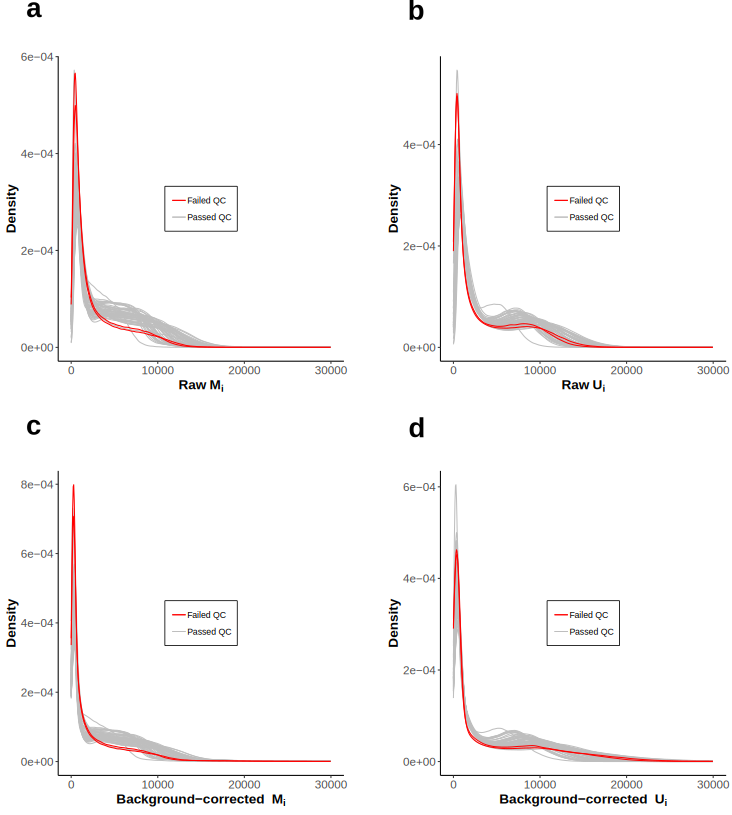
\includegraphics[width=0.62\textwidth]{SC2_Fig1}
	\caption[Effects of \textit{noob} background correction on the array fluorescence intensities.]{Effects of \textit{noob} background correction on the array flurescence intensities. Distributions of the array fluorescence intensities for the \textbf{a.} methylated signals ($M_{i}$) before background correction; \textbf{b.} unmethylated signals ($U_{i}$) before background correction; \textbf{c.} methylated signals ($M_{i}$) after background correction and \textbf{d.} unmethylated signals ($U_{i}$) after background correction. Each curve represents a DNA methylation sample from the GSE41273 batch. In grey: 51 samples that passed quality control (QC). In red: 2 samples that failed QC.}
	\label{fig:sc2_fig1}
\end{figure}

\begin{figure}[htbp!] 
	\centering    
	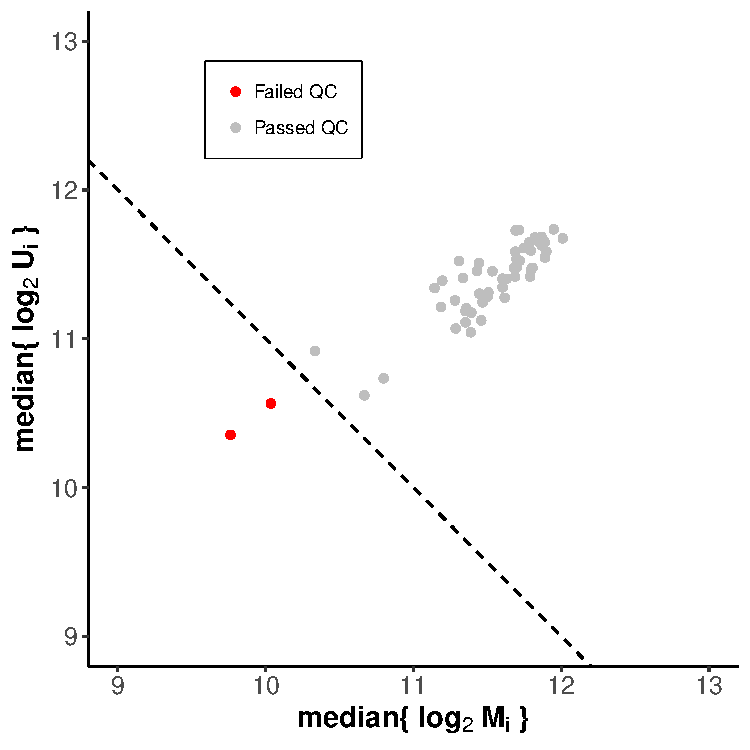
\includegraphics[width=0.5\textwidth]{SC2_Fig2}
	\caption[Quality control (QC) strategy to identify outlier samples.]{Quality control (QC) strategy to identify outlier samples, according to their global intensity values, in the GSE41273 batch. Those samples with low median intensity values (see criteria in the main text) were discarded from downstream analyses (2/53, in red). Each sample is represented by one point. The dashed line represents the  intensity threshold. $M_{i}$ and $U_{i}$ represent the background-corrected methylated and unmethylated intensity measurements for all the 450K array probes in a given sample.}
	\label{fig:sc2_fig2}
\end{figure}

\begin{figure}[htbp!] 
	\centering    
	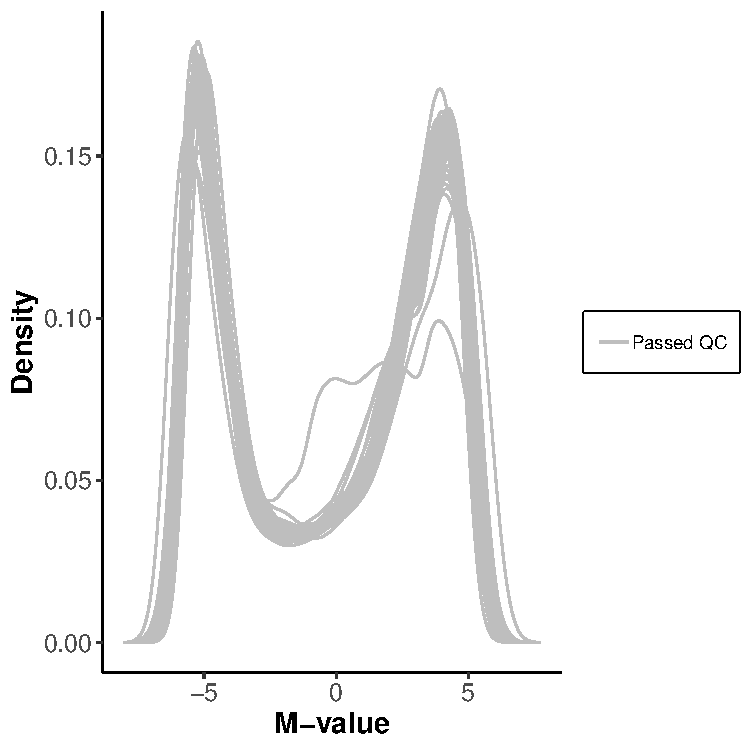
\includegraphics[width=0.5\textwidth]{SC2_Fig3}
	\caption[M-value distributions in the GSE41273 batch]{M-value distributions in the samples of the GSE41273 batch, after all the pre-processing steps have been carried out (background correction, quality control, probe filtering and BMIQ normalisation). M-values were calculated applying the logistic transformation to the $\beta$-values, as described in Du \textit{et al.} \cite{Du2010}. Each curve represents a different sample.}
	\label{fig:sc2_fig3}
\end{figure}





\smallskip

\renewcommand{\thesection}{S.2}   
\section{Biological aspects of the epigenetic clock}

\renewcommand\thefigure{S2.\arabic{figure}}    
\bigskip

\smallskip

\clearpage

\renewcommand{\thesection}{S.3}   
\section{Technological aspects of epigenetic clocks}

\renewcommand\thefigure{S3.\arabic{figure}}    
\bigskip

\begin{figure}[htbp!] 
	\centering    
	\setcounter{figure}{0}
	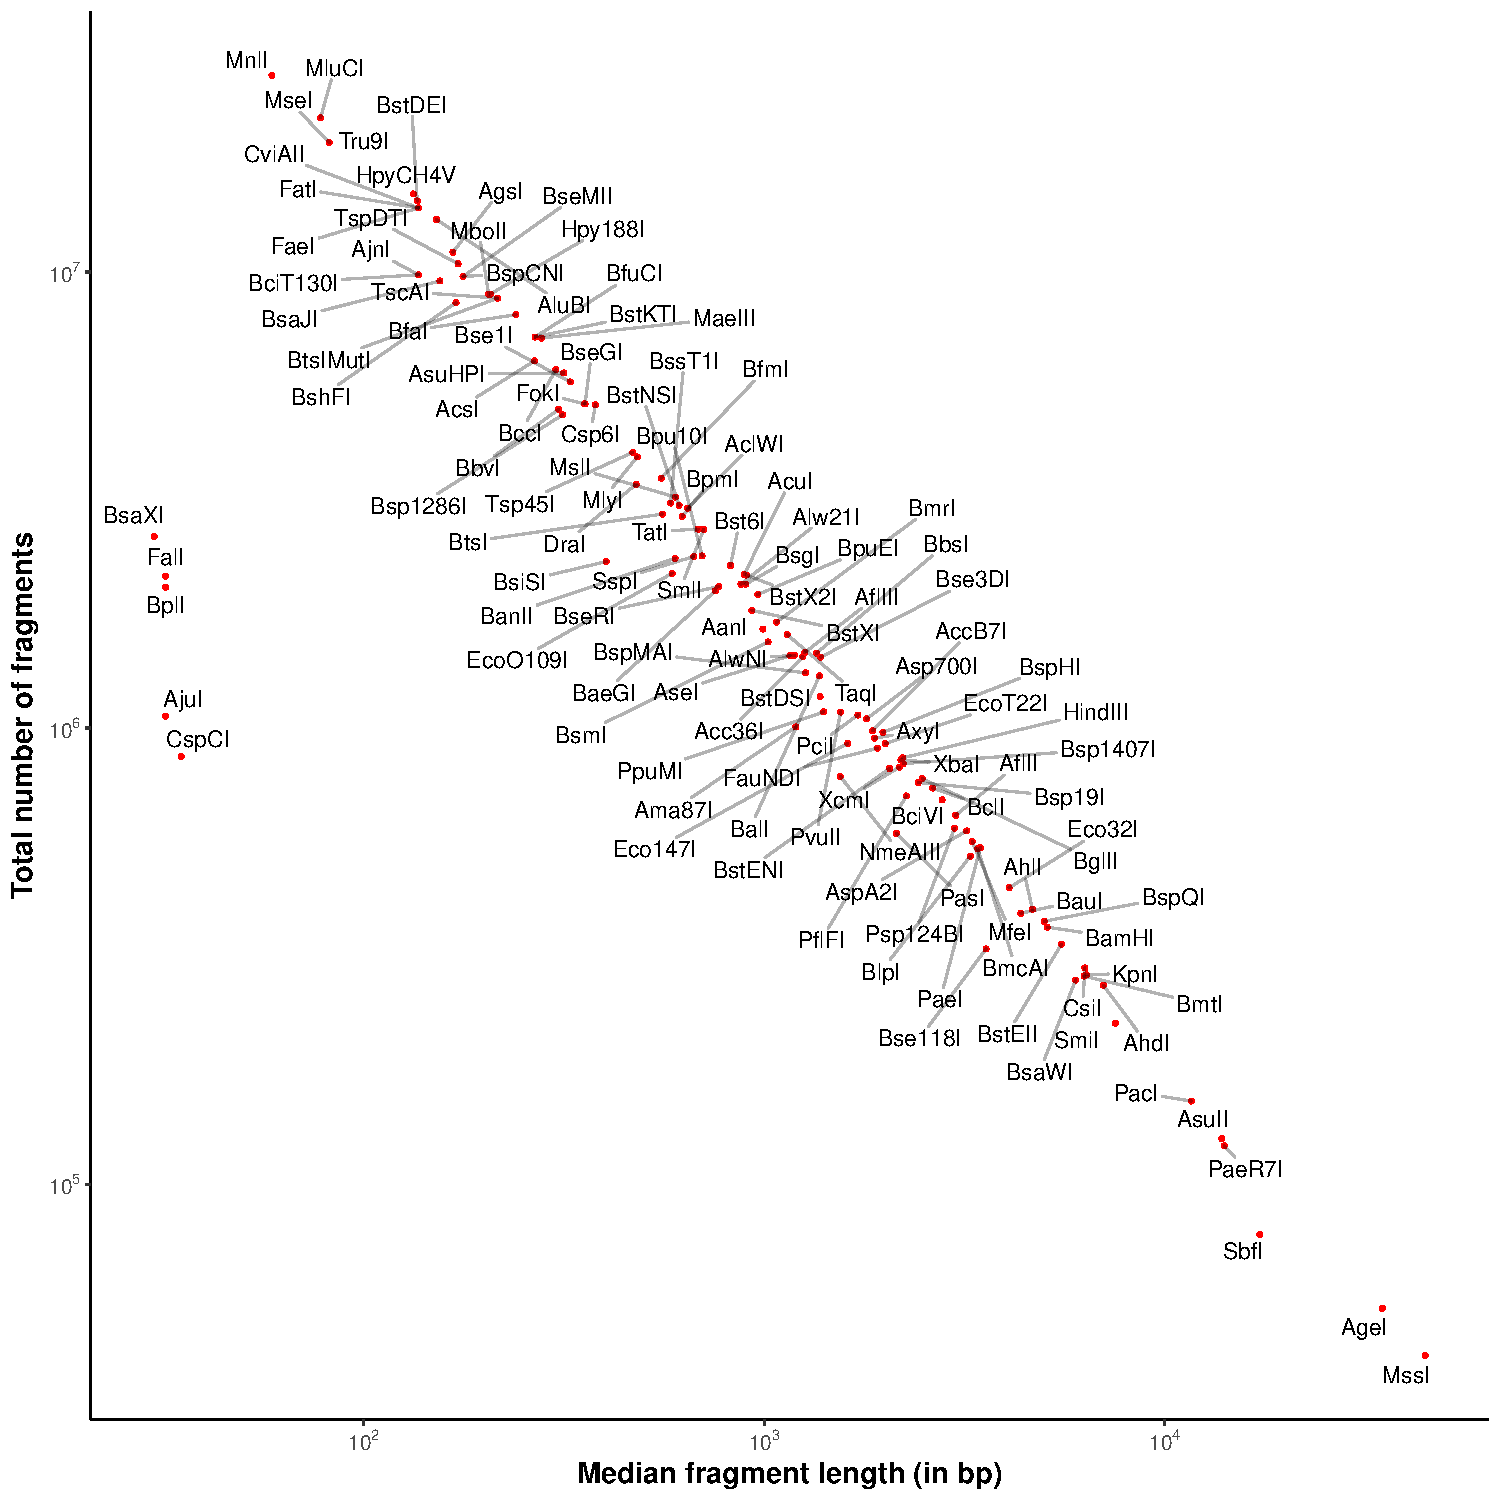
\includegraphics[width=0.7\textwidth]{SC4_Fig1}
	\caption[Scatterplot of fragment length distributions for the isoschizomer families]{Scatterplot which summarises the fragment length distributions for the same isoschizomer families portrayed in Fig~\ref{fig:c4_fig2}a. The red dots represent the actual values of median fragment length and total number of fragments for each family. The black lines assign each name label to the correspondent red point for visualization purposes.}
	\label{fig:sc4_fig1}
\end{figure}

\begin{figure}[htbp!] 
	\centering    
	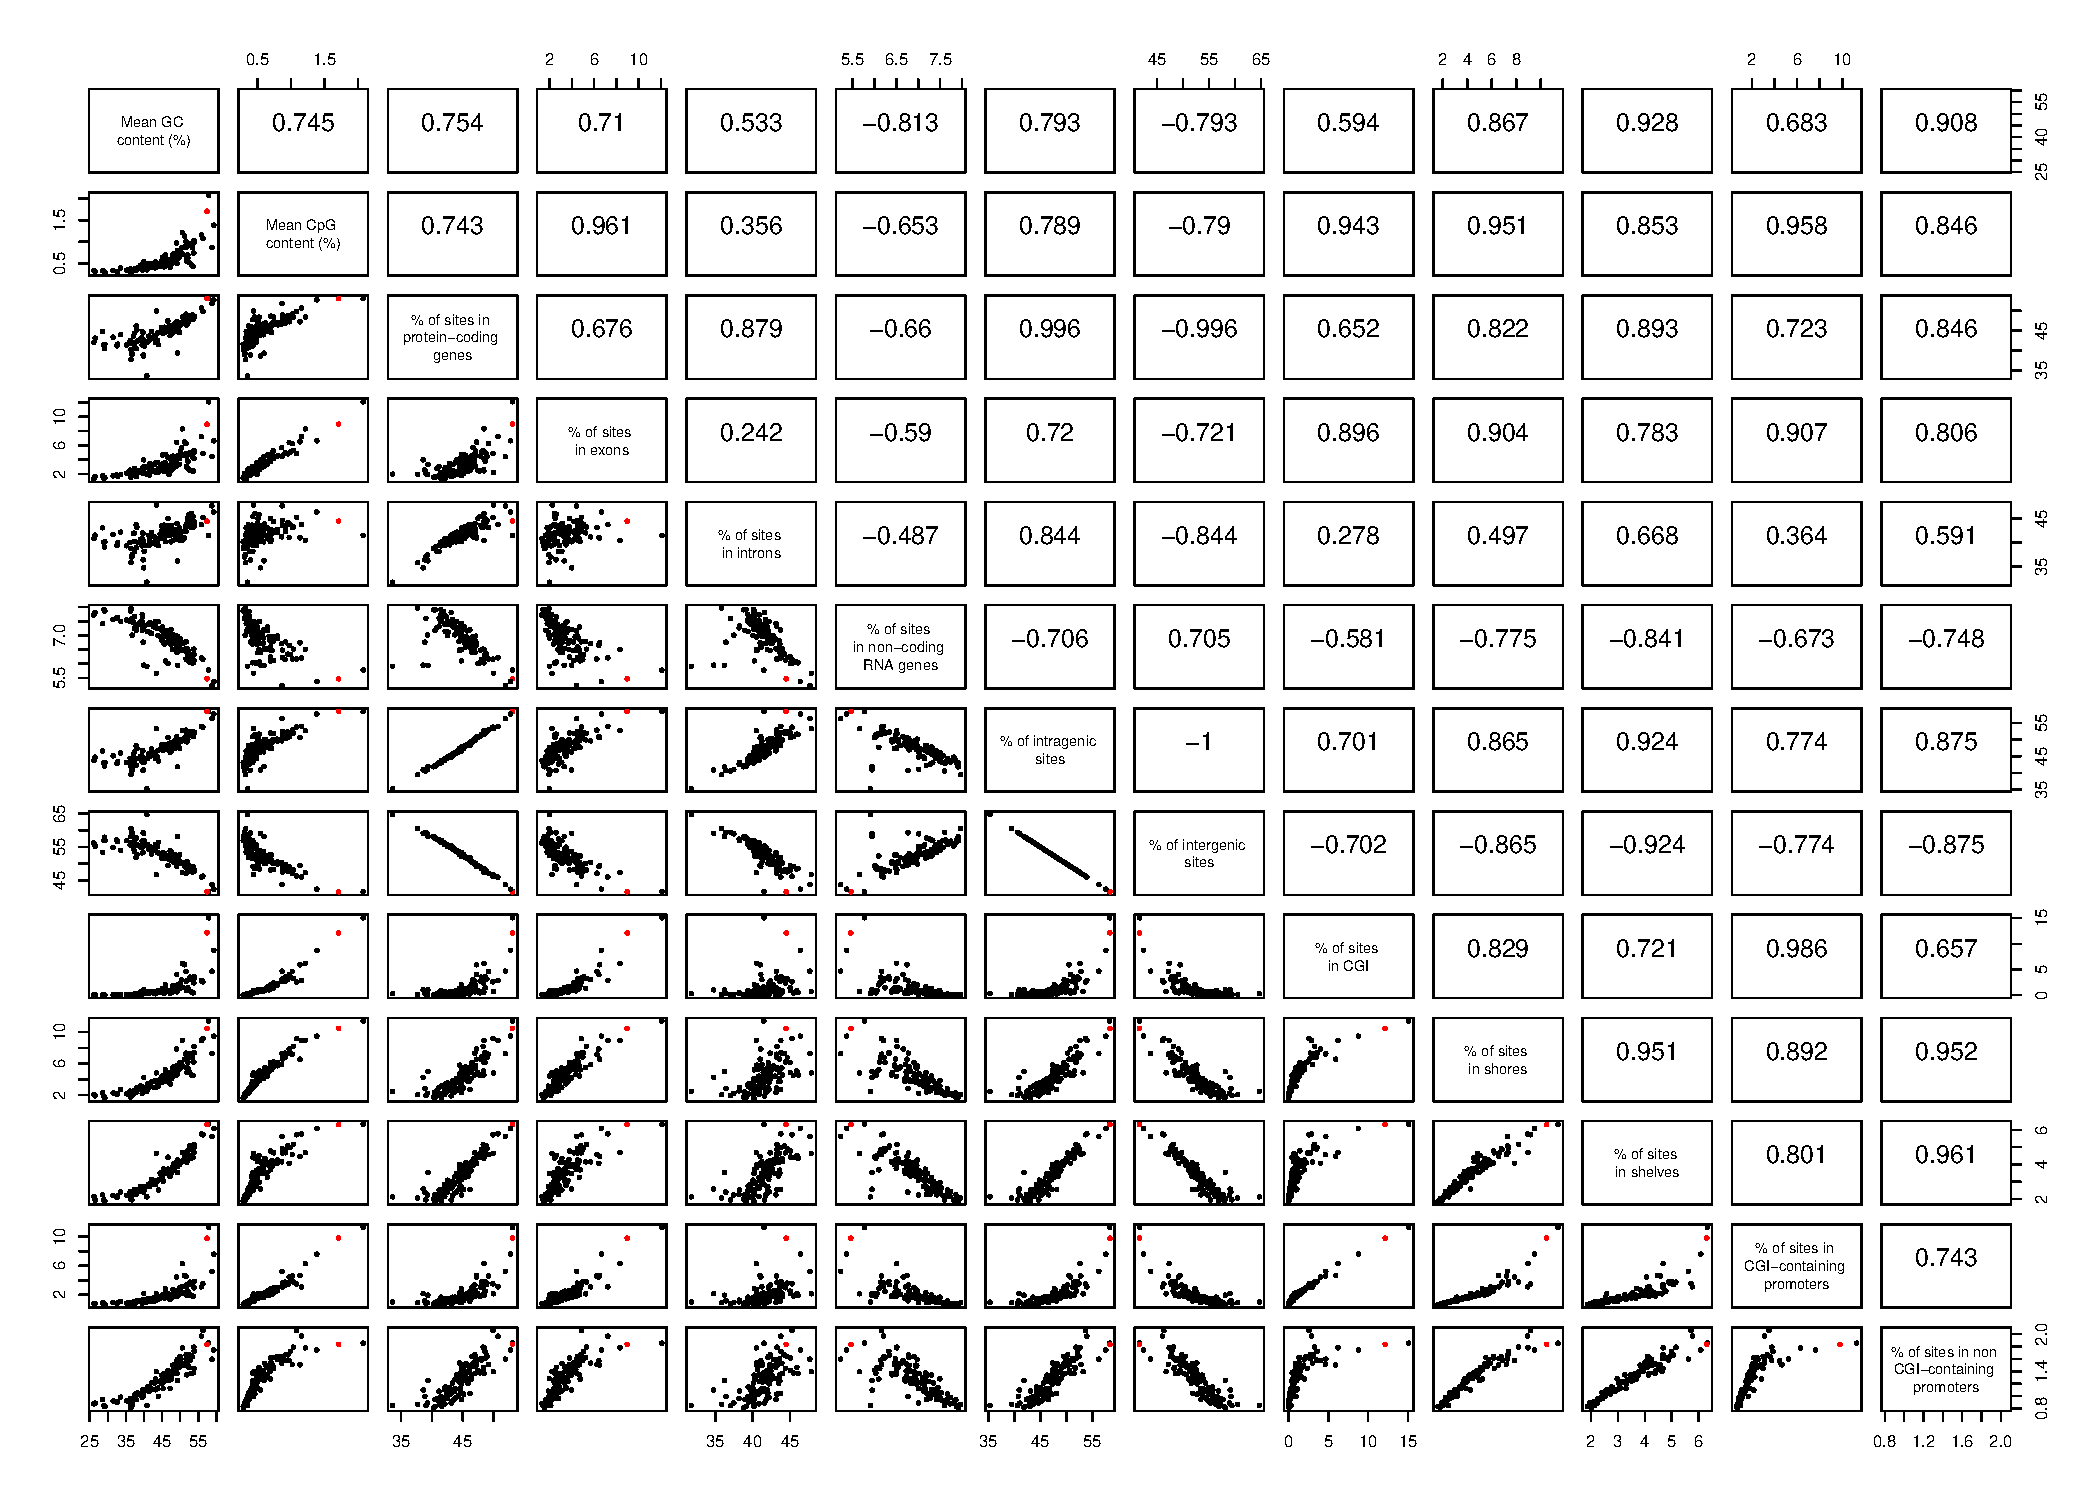
\includegraphics[width=1\textwidth]{SC4_Fig2}
	\caption[Genomic features that overlap with restriction enzyme cleavage sites]{Matrix of scatterplots showing the percentages of cleavage sites from different restriction enzymes that overlap with several genomic features (listed on the diagonal) in the human genome (hg38). The red dot in each scatterplot represents the values for MspI. The numbers above the diagonal are the Pearson correlation coefficients between all the possible pairs of genomic features.}
	\label{fig:sc4_fig2}
\end{figure}

\begin{figure}[htbp!] 
	\centering    
	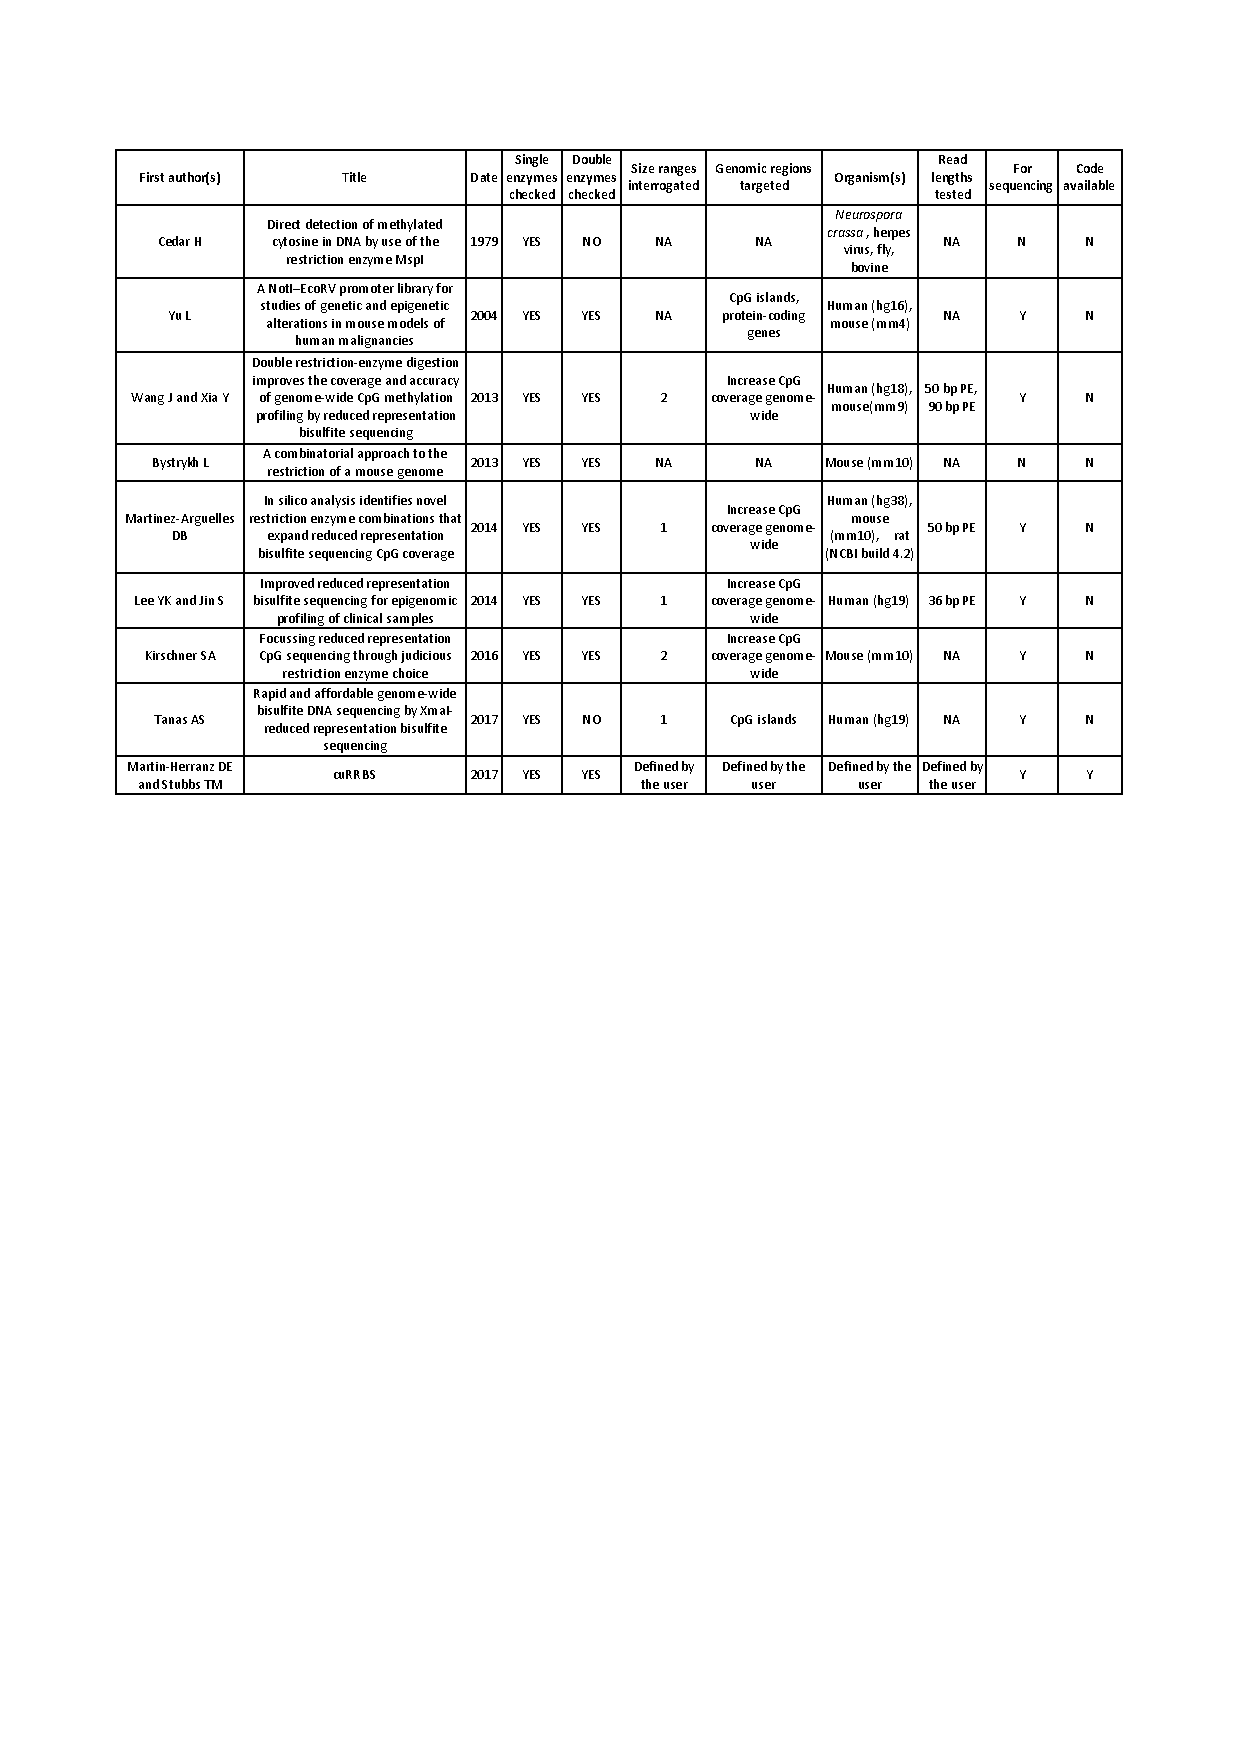
\includegraphics[width=1.0\textwidth]{SC4_Fig3}
	\caption[Comparison of studies using restriction enzymes for genomic enrichment]{Table showing the comparison of different studies that have attempted to use restriction enzymes to target different regions in the genome.}
	\label{fig:sc4_fig3}
\end{figure}

\begin{figure}[htbp!] 
	\centering    
	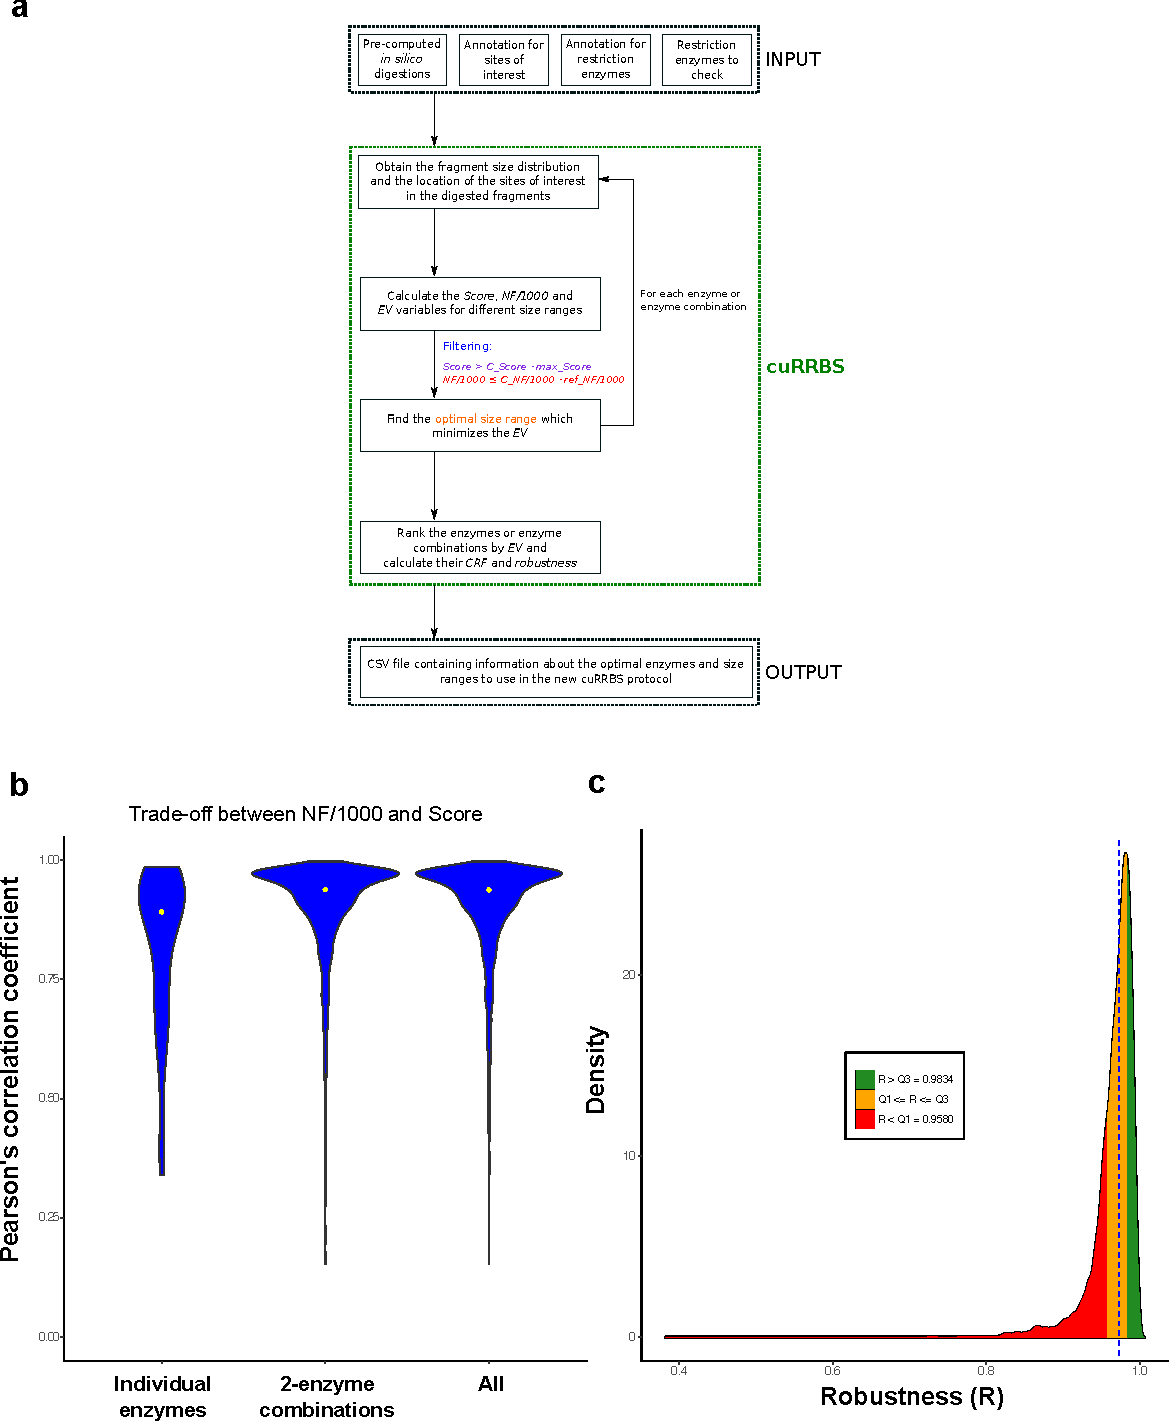
\includegraphics[width=1.0\textwidth]{SC4_Fig4}
	\vspace*{1mm}
	\caption[Additional insights into cuRRBS]{Additional insights into cuRRBS. \textbf{a.} Detailed flowchart showing the input, main steps in cuRRBS and the output of the software. \textbf{b.} Violin plots showing the distribution of Pearson's correlation coefficients between the number of fragments (\textit{NF}) and the \textit{Score} for all the different enzymes tested with cuRRBS (single-enzyme, double-enzyme, all). In this example we used the Horvath epigenetic clock system \cite{Horvath2013}, checking all the \textit{size ranges} between 20 and 1000 bp, with an \textit{experimental error} of 10 bp and a \textit{read length} of 75 bp. Each yellow point represents the median for the Pearson's correlation coefficients under consideration. \textbf{c.} Density plot showing the distribution of the \textit{robustness} (\textit{R}) values when assuming an \textit{experimental error} ($\delta$) of 20 bp. cuRRBS was run for all the biological systems under study (Fig.~\ref{fig:sc4_fig5}) \cite{Horvath2013,Hanna2016,Milagre2017,Kawakatsu2016,Maurano2015,LevMaor2015,Domcke2015} with the same parameters as described in `Running cuRRBS for different \textit{in silico} systems' (all the hits that satisfied the \textit{thresholds} were reported in this case). The dashed blue line represents the median (0.9734). The different colours provide a way to judge the \textit{robustness} values: bad (in red, $R < Q_1 = 0.9580$), medium (in orange, $Q_1 \leq R \leq Q_3 = 0.9834$) and good (in green, $R > Q_3$); where $Q_1$ and $Q_3$ represent the first and the third quartiles respectively.}
	\label{fig:sc4_fig4}
\end{figure}

\begin{figure}[htbp!] 
	\centering    
	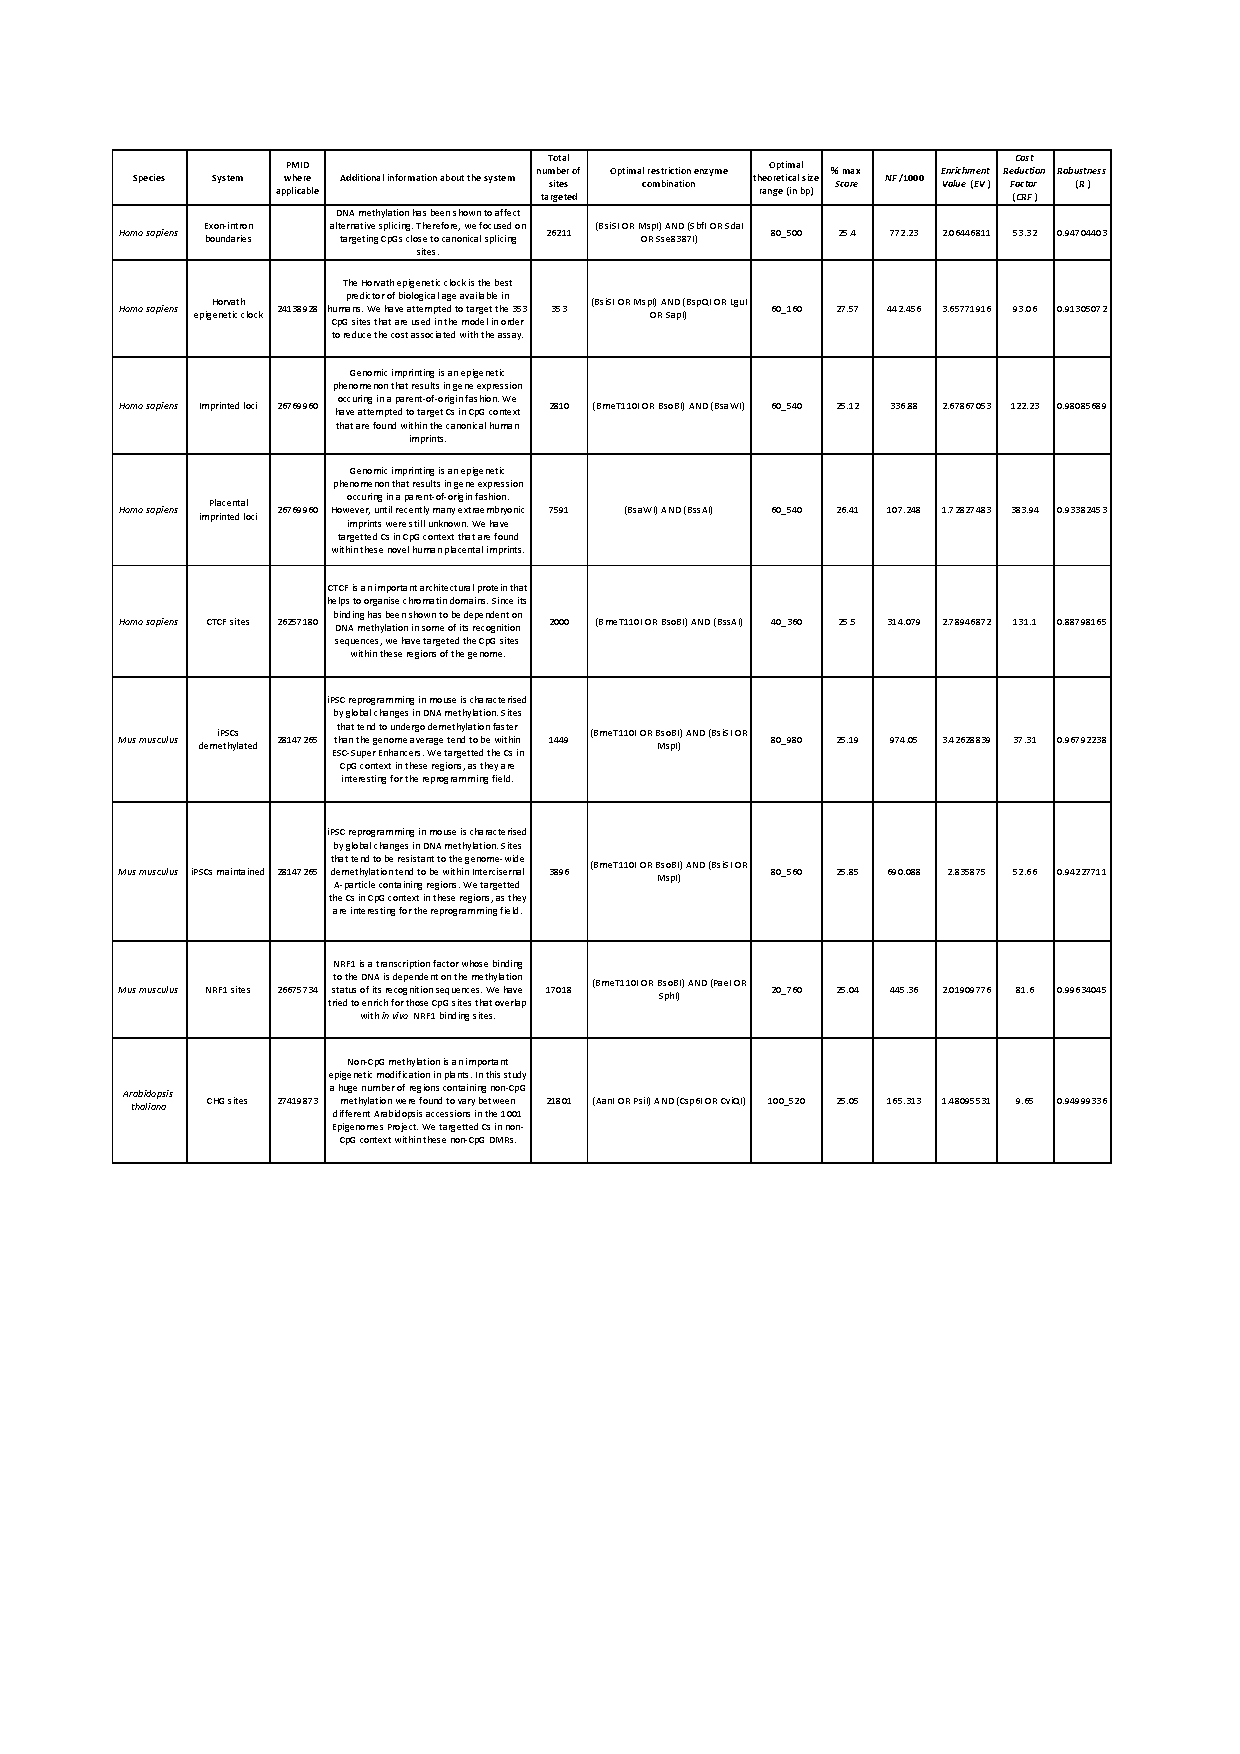
\includegraphics[width=1.0\textwidth]{SC4_Fig5}
	\caption[Additional results of running cuRRBS in different biological systems]{Table showing the information regarding the different biological systems \cite{Horvath2013,Hanna2016,Milagre2017,Kawakatsu2016,Maurano2015,LevMaor2015,Domcke2015} for which cuRRBS was run \textit{in silico}. Some variables from the top hits in cuRRBS output are also reported.}
	\label{fig:sc4_fig5}
\end{figure}

\begin{figure}[htbp!] 
	\centering    
	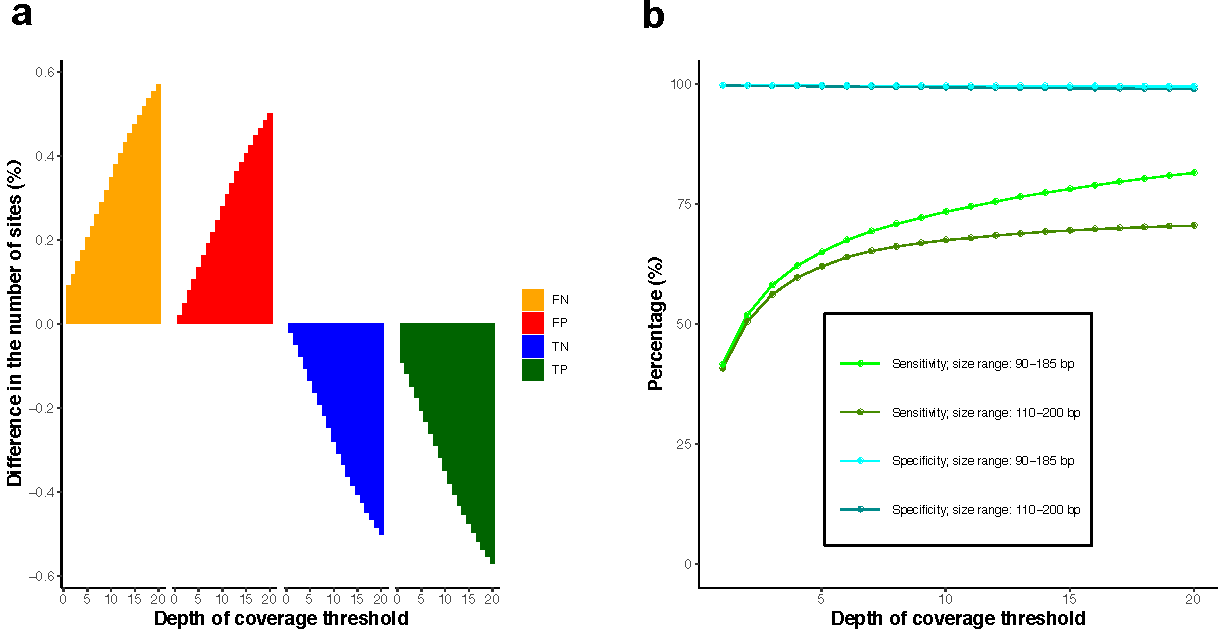
\includegraphics[width=1.0\textwidth]{SC4_Fig6}
	\vspace*{2mm}
	\caption[Effect of experimental errors during size selection in cuRRBS predictions]{Effect of experimental errors during size selection in cuRRBS predictions. \textbf{a.} Barplots showing the difference in the number of true positives (TP, in green), true negatives (TN, in blue), false positives (FP, in red) and false negatives (FN, in yellow) derived from cuRRBS theoretical predictions for the XmaI-RRBS data \cite{Tanas2017} using two different size ranges: 110-200 bp (aimed size range) and 90-185 bp (real size range). The difference observed between the two size ranges (aimed - real) is expressed as the percentage of the total number of sites considered (i.e. all CGI- CpGs). The number of sites in each category is calculated for different thresholds in the depth of coverage (number of reads covering a CpG site as reported by Bismark). cuRRBS was run for XmaI with all the default parameters (with a \textit{read length} of 200 bp). Legend is displayed on the right hand side. \textbf{b.} Plot showing values of cuRRBS sensitivity and specificity as a function of the depth of coverage threshold employed to filter the experimental data \cite{Tanas2017}. The two size ranges considered in a. (aimed: 110-200 bp; real: 90-185 bp) are used for the calculations. Legend is displayed below the plot curves.}
	\label{fig:sc4_fig6}
\end{figure}

\begin{figure}[htbp!] 
	\centering    
	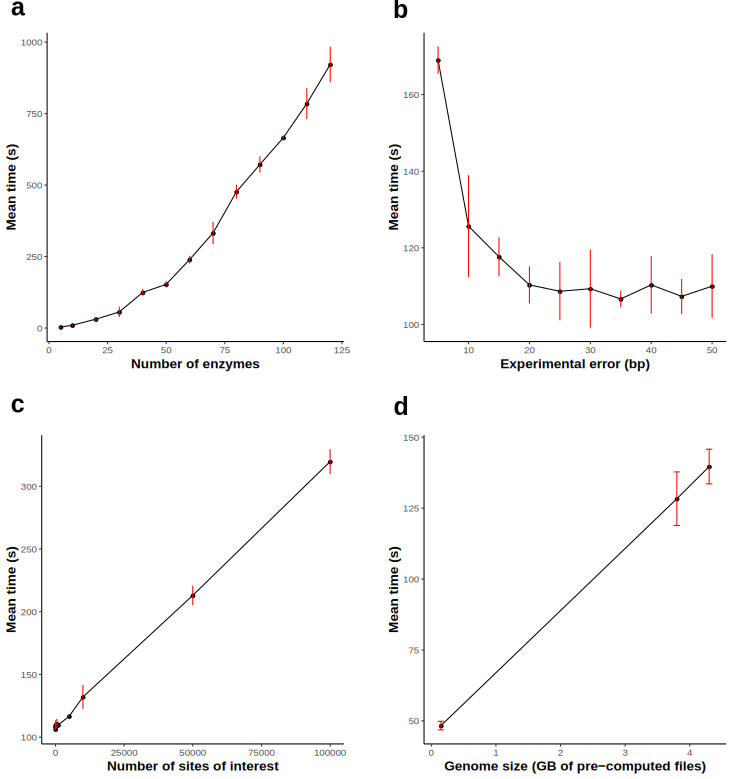
\includegraphics[width=0.8\textwidth]{SC4_Fig7}
	\vspace*{1mm}
	\caption[cuRRBS computational efficiency]{cuRRBS computational efficiency. \textbf{a.} Plot showing the dependency between the number of enzymes checked and the computational (real) time required by the software (mean between 3 independent runs). cuRRBS was run for the Horvath epigenetic clock system \cite{Horvath2013} with a \textit{read length} of 75 bp, a \textit{Score threshold} of $25\%$ and an \textit{experimental error} of 10 bp. A laptop with an Intel® Core$^{TM}$ i7-6600U CPU was used, which allowed cuRRBS to employ 4 parallel threads. The red error bars display the mean ± \acrshort{SD} for the 3 independent runs. \textbf{b.} Plot showing the dependency between the \textit{experimental error} (which determines how many size ranges are sampled) and the computational (real) time required by the software (mean between 3 independent runs). cuRRBS was run for the Horvath epigenetic clock system \cite{Horvath2013} with a \textit{read length} of 75 bp, a \textit{Score threshold} of $25\%$ and a list with 40 enzymes. A laptop with an Intel® Core$^{TM}$ i7-6600U CPU was used, which allowed cuRRBS to employ 4 parallel threads. The red error bars display the mean ± SD for the 3 independent runs. \textbf{c.} Plot showing the dependency between the number of sites of interest and the computational (real) time required by the software (mean between 3 independent runs). cuRRBS was run with a \textit{read length} of 75 bp, a \textit{Score threshold} of $25\%$, an \textit{experimental error} of 10 bp and a list with 40 enzymes. A laptop with an Intel® Core$^{TM}$ i7-6600U CPU was used, which allowed cuRRBS to employ 4 parallel threads. The red error bars display the mean ± SD for the 3 independent runs. \textbf{d.} Plot showing the dependency between genome size (measured as the size in GB of all the pre-computed files) and the computational (real) time required by the software (mean between 3 independent runs). cuRRBS was run with a \textit{read length} of 75 bp, a \textit{Score threshold} of $25\%$, an experimental error of 10 bp and a list with 40 enzymes. A laptop with an Intel® Core$^{TM}$ i7-6600U CPU was used, which allowed cuRRBS to employ 4 parallel threads. The red error bars display the mean ± SD for the 3 independent runs.}
	\label{fig:sc4_fig7}
\end{figure}


